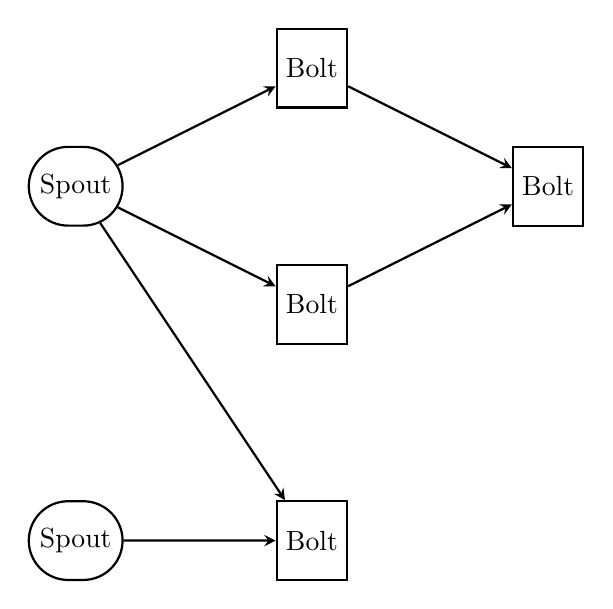
\begin{tikzpicture}[>=stealth]
	\usetikzlibrary{shapes}
	\node (spout0)			at (0,2.5) [rounded rectangle, draw, minimum height=1cm,thick] {Spout};
	\node (spout1)			at (0,-2) [rounded rectangle, draw, minimum height=1cm,thick] {Spout};

	\node (bolt0)			at (3,4) [rectangle, draw, minimum height=1cm,thick] {Bolt};
	\node (bolt1)			at (3,1) [rectangle, draw, minimum height=1cm,thick] {Bolt};
	\node (bolt2)			at (3,-2) [rectangle, draw, minimum height=1cm,thick] {Bolt};

	\node (bolt3)			at (6,2.5) [rectangle, draw, minimum height=1cm,thick] {Bolt};


	\path (spout0)		edge[->,thick] (bolt0)
		(spout0)				edge[->,thick] (bolt1)
		(spout0)				edge[->,thick] (bolt2)
		(spout1)				edge[->,thick] (bolt2)
		(bolt0)	  			edge[->,thick] (bolt3)
		(bolt1)	  			edge[->,thick] (bolt3);
\end{tikzpicture}
